\documentclass[11pt,twocolumn]{article}
\usepackage[utf8]{inputenc}
\usepackage[english]{babel}
\usepackage{pdfpages}
\usepackage{hyperref}
\usepackage{float}
\usepackage{verbatim}
\usepackage{balance}
\usepackage{graphicx}

\title{Network Analysis in ArangoDB}
\date{January 2020}
\author{Alessandro d'Agostino, Mattia Ceccarelli, Riccardo Scheda}

\begin{document}

\twocolumn[
\begin{@twocolumnfalse}

\maketitle

\begin{abstract}
The project aim is to develop a simple python API that let the user interact with the open-source multi-model database ArangoDB to perform fast queries on multi-partite graphs, extract and visualize sub-network which can then be analized with powerful python libraries.
The study also includes results on the computational efficiency of ArangoDB's algorithms, in order to have an estimate of the API timing behaviours with large networks.
\end{abstract}
\end{@twocolumnfalse}
]

\section{Introduction}
ArangoDB \cite{WEBSITE:arangodb} is a multi-model, open-source database with flexible data models for documents, graphs and key-values. It is being used in different fields: from semantic analysis to genome studies.

In the present work we employed the library \texttt{python-arango}  \cite{WEBSITE:pythonarango} to import and export multipartite network-like databases, that are defined as collections of documents (nodes) and collections of relationships between them (edges).

In particular, a document is a python dictionary with a mandatory  \texttt{\_id}  key assigned to a unique value.
What we call an "edge" is also a python dictionary, but with an  \texttt{\_id} ,  \texttt{\_source} and  \texttt{\_target}  voices, to specify not only the linked nodes, but also the direction of said link in the case of directed graphs.

\paragraph{Graph Object}
A Graph is the combination of at least one node collection and one or multiple edge collections, called edge definitions.
With a Graph two main operations are available: visualization and execution of queries.

The former is possible thanks to ArangoDB web interface, as shown in the figures below, which provide the user many options such as the starting node and the number of elements to load. By default, the starting node is random.

For the latter we relied on the poweful AQL, that is the query language implemented in arango. It is used to execute different kind of "search" through the graph, and select nodes and edges.

\paragraph{Why ArangoDB?}
ArangoDB resulted to be the NoSQL engine with the most favorable compromise between memory usage and computation speed among others available alternatives. A comparative table of the performance of different NoSQL engines is reported in figure \ref{fig:tab}.
ArangoDB offers a valid web interface where all the commands can be given intuitively and graph and queries' results can be visualized in an organic way.
Furthermore there are several ArangoDB Python interfaces available on line, which allowed us to taylor this poweful tool to our needs.

\begin{figure}[ht!]
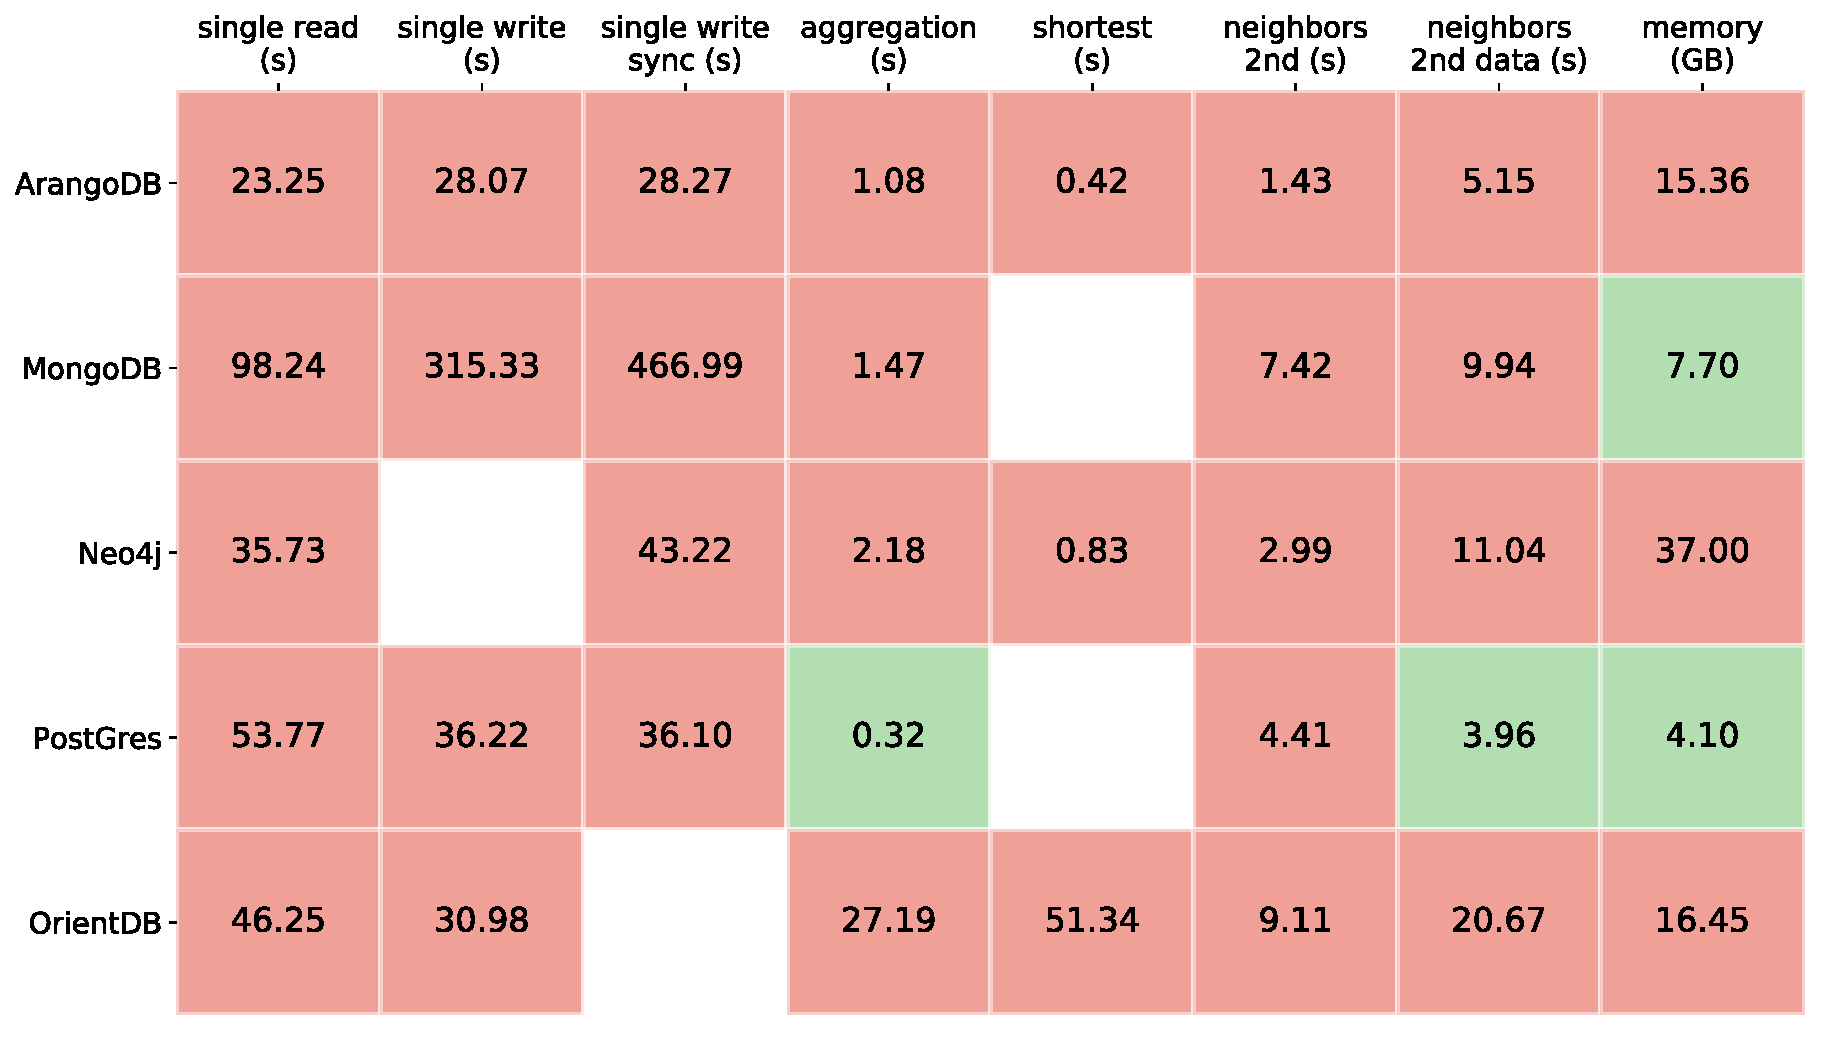
\includegraphics[width=\columnwidth]{images/arango_perf.pdf}
\caption{\small{\textit{Comparison between time performances of different NoSQL engines for some common operation. ArnagoDB shows the overall best results. }}}
\label{fig:tab}
\end{figure}

\paragraph{NetworkX}
Even though ArangoDB allows fast queries it is necessary the right tool to study the characteristics of a resulting subnet. For this purpose we decided to exploit mainly the Python library NetworkX \cite{WEBSITE:networkx} due to its huge availability of function and tools.

\section{Pipeline}
Now we describe a typical usage case and all the operations needed to extract a subgraph in ArangoDB.
The first thing to do is to read the file in the right input format (typically \texttt{.gexf}) through the dedicated function \texttt{read\_gexf}:

\begin{verbatim}
ArDB_Net, Nx_Net =
  read_gexf(db,
            filename,
            nodes_collection_name='nodes',
            edges_collection_name='edges',
            graph_name='Net',
            multipartite=False)
\end{verbatim}

The function takes the information about nodes and edges from the gexf file and creates the corrispondent collections on ArangoDB.
Then it returns two graphs: one of python-arango type and one of networkx type.

Once the graph and the collections of nodes and edges are uploaded on Arango web interface we can proceed with futher analysis. For instance, we can perform a graph traversal aimed to extract the first neighbours of a certain node.

In this case we can make use of python-arango, calling the function:

\begin{verbatim}
first_neighbours = traverse(db,
         starting_node,
         nodes_collection_name,
         graph_name,
         direction='outbound',
         item_order='forward',
         min_depth=0,
         max_depth=1,
         vertex_uniqueness='global')
\end{verbatim}

Tuning the given parameters, any traversal could be performed. The output of this type of function is meant to be the resulting sub net saved as Python dictionaries containing vertexes and paths crossed by the traverse.

Having the list of the first neighbours we can obtain the corresponding subnet just using the function \texttt{subgraph} given by Networkx:

\begin{verbatim}
Nx_Sub_Net =
        Nx_Net.subgraph([vertex['label']
        for vertex in
        first_neighbours['vertices']])
\end{verbatim}

In this way we create the minimal subgraph containing only the nearest neighbours of the selected node with the labels of nodes and the corresponding edges.
To recover every information contained in the starting network, we add all the attributes back to each node:

\begin{verbatim}
for node in Nx_Sub_Net:
  attr = pa.get_vertex(db,
                       {'label':node},
                        'Sym_Deas')
  nx.set_node_attributes(Nx_Sub_Net,
                        {node : attr})
\end{verbatim}

The last thing to do is to import the subnet in ArangoDB, using the two specific functions  \verb nx_to_arango  and \verb export_to_arango , for this passage is easier to convert the data in the node\_link\_data format:

\begin{verbatim}
sub_net =
  nx.readwrite.node_link_data(Nx_Sub_Net)
sub_net =
  pa.nx_to_arango(sub_net, 'Sub_Net')
Sub_Net = pa.export_to_arango(db,
                  msub_net,
                  'Sub_Net',
                  'Sub_Net_edges',
                  'Sub_Graph')
\end{verbatim}

Now the resulting subnet is ready for every kind of analysis offered by NetworkX.
This is a useful procedure to extract articulated subnets.

\section{Timing}
As already mentioned, one of the main focuses is to apply queries to very big networks.
Therefore a study on how the time spent to perform a query scales with graph's dimension was necessary.
Hence we chose two different queries to be performed on several graphs with similar characteristics but increasing dimensions.

The queries taken into consideration are the traversal that extract the second neighbours (\verb min_depth=0  \verb max_depth=2 ) and the first four shortest path between two random nodes .

We created random graphs with a number of nodes ranging from 100 to 10000, using the NetworkX function \verb fast_gnp_random_graph .
One important factor is the number of links: infact, a dense networks with such an high number of nodes is impossible to handle for a home computer.
So, we chose to generate random graphs with $\rho = 0.075$, which comes from the analysis of the real case we tested the algorithms on.

We runned the queries under study onto 30 different starting nodes, in order to obtain an average value, its deviation and a idea of its trend.

\section{Results}

In the following section, we present the data obtained for timing, and an example on the visualization of a network and a sub-network through ArangoDB web interface.

\paragraph{Performances}
In figure \ref{fig:sh_paths} we present the trend of times with respect to number of nodes, for the algorithm that find the 4 shortest paths between two nodes. We performed a linear fitting on the sampled data and a polynomial fit of degree 2, the latter seems to be the best result with $R^2 = 0.975$.

In figure \ref{fig:tr_0_2}, we show the trend of times with respect to the dimensions of the network for the traversal that extract the second order neighbours of a chosen node. We performed a linear fitting and a polynomial fit of degree 2, even in this case the best fit result from the polynomial one, with $R^2 = 0.968$.

From the analysis of both the two different Benchmark series we found that the time took by the queries apparently scales quadratically with the graph dimension.
This is a useful information and it allows to make prediction based on the particular graph under analysis.

\begin{figure}[ht!]
  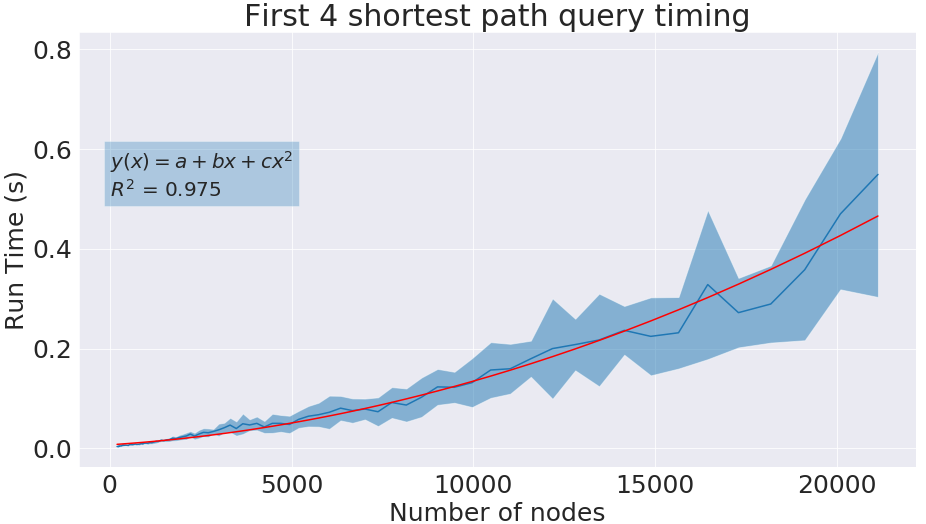
\includegraphics[width=\linewidth]{images/4_shortest_path_timing_poly.png}
  \caption{\small{\textit{Timing trend for the query that extracts the first 4 shortest paths between two random nodes. The mean is computed for 30 different couples on the same graph.}}}
  \label{fig:sh_paths}
\end{figure}

\begin{figure}[ht!]
   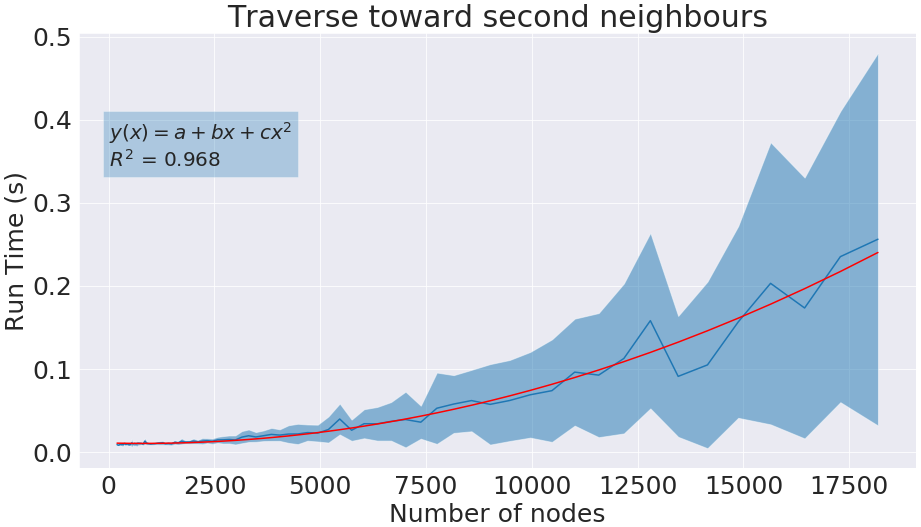
\includegraphics[width=\linewidth]{images/traverse_0_2_poly.png}
   \caption{\small{\textit{Timing trend of the second neighbours extraction query. The mean is calculated for 30 different starting nodes on the same graph.}}}
   \label{fig:tr_0_2}
\end{figure}

\newpage

\paragraph{Visualization}
In figure \ref{fig:3} we show an example of visualization of a random branch of the network used as testing ground for the API.

\begin{figure}[ht!]
   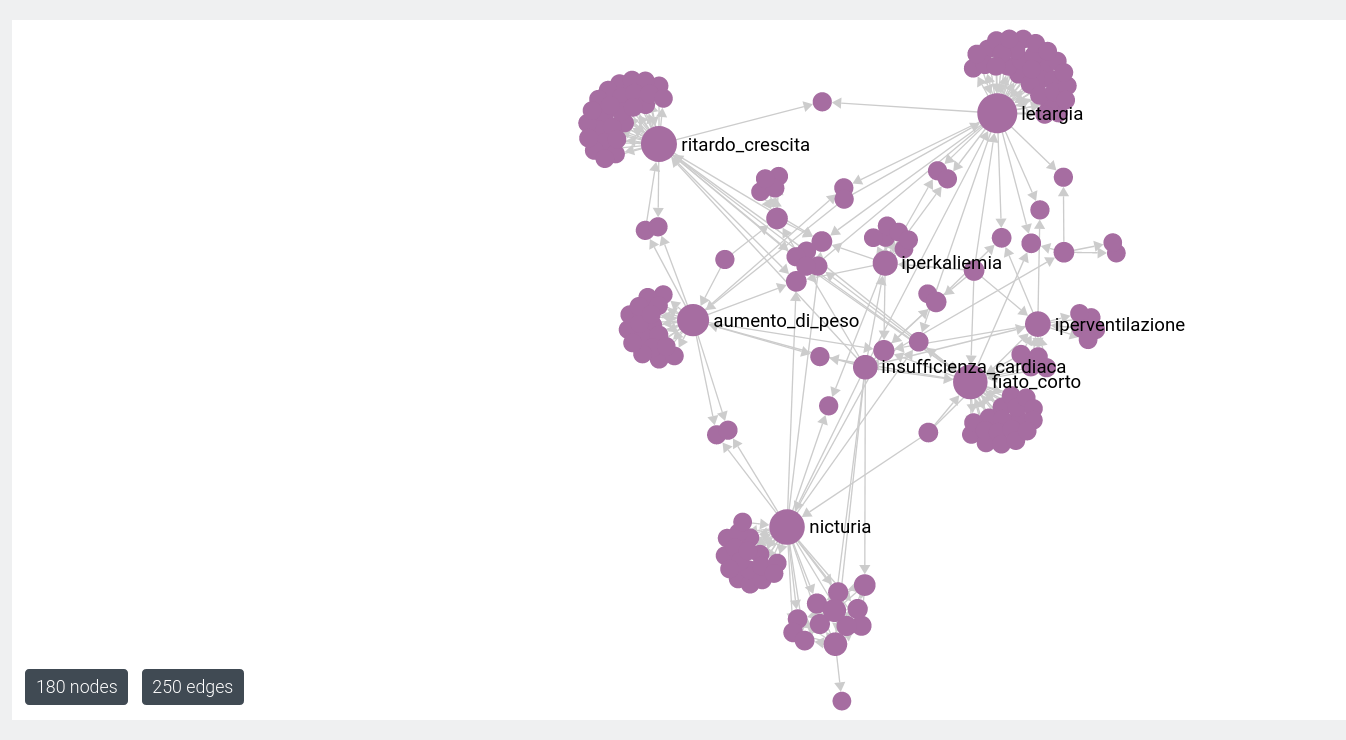
\includegraphics[width=\linewidth]{images/Sym_Net_crop.png}
   \caption{\small{\textit{ArangoDB visualization tool: in this figure we show a random branch of SymptomsNet, a graph of symptoms and diseases.}}}
   \label{fig:3}
\end{figure}

In figure \ref{fig:4}, instead, the subnetwork of the nearest neighbours of the nodes with label \textit{emicrania} is shown, extracted using the pipeline descripted above.

\begin{figure}[ht!]
   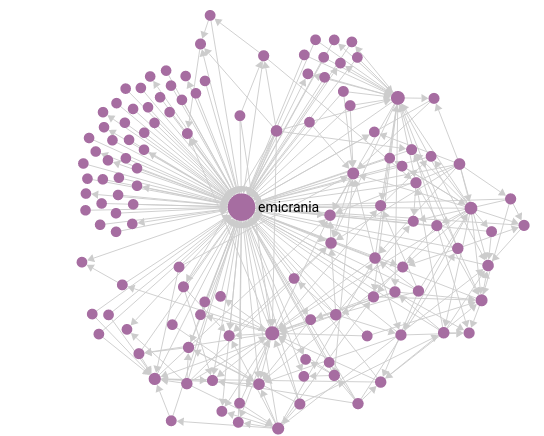
\includegraphics[width=\linewidth]{images/neigh_emicrania.png}
   \caption{\small{\textit{ArangoDB visualization tool: in this figure we show the network of first neighbours of \textit{emicrania} (cronic headache).}}}
   \label{fig:4}
\end{figure}

In the case of a multipartite graph, objects from different classes can be visualized with different colours.

\newpage

\section{Conclusions}
\balance % ci sta
We've produced an applicative to visualize and efficiently query a graph-like database with a simple yet resourceful programming language like python.

As shown in the results, the scaling of the ArangoDB query algorithm seems quadratic for the two cases taken into consideration, $k$ shortest paths and neighborhood search.

\paragraph{Open Problems}

The main problems lay in the level of control we can gather through python. Indeed, it seems to be impossible to load and save default queries.
Moreover, we couldn't manage to save graph visualization options, which could ease the accessibility.

Another issue, comes from the slowness of the exportation to arango algorithm, but since it is a \textit{una tantum} operation, hence not a priority.

\paragraph{Future Ideas}

We will focus on preparing the applicative for the non-programmer user.

We think a Graphical User Interface (GUI) could greatly smoothen the user experience.

In the future we want to test the applicative with a much larger database than the one we had at disposal.

\twocolumn[
\begin{@twocolumnfalse}
\bibliography{biblio}
\bibliographystyle{ieeetr}
\end{@twocolumnfalse}
]

\end{document}
